% called by main.tex
%
\chapter{Estado del arte}
\label{ch::chapter2}

El desarrollo de este trabajo se enmarca en los esfuerzos impulsados por \textbf{NIST} 
para estandarizar algoritmos criptográficos resistentes a ataques cuánticos. 

En las fases iniciales del proyecto, se realizó un análisis comparativo de las propuestas 
criptográficas consideradas en la cuarta ronda del proceso de estandarización de 
\textbf{NIST}. Como resultado de este análisis, se seleccionó el esquema \textbf{HQC} 
como el esquema estudiado. Posteriormente, la selección de \textbf{HQC} 
por parte de \textbf{NIST} en marzo de 2025, reforzó su interes de an alizar su comportamiento
en plataformas IoT. 

Este capitulo se presenta como una revisón del estado del arte en el campo de la criptografía 
post-cuántica. En primer lugar, se introduce los conceptos esenciales de criptografía clásica y 
post-cuántica, prestando atencion a los mecanismos de encapsulación de claves y al esquema HQC.
A continuacion, se describen las principales caracteristicas y limitaciones de las redes IoT que 
condicionan la incorporación de esquemas criptográficos post-cuánticos.
Finalmente, se revisan los trabajos erlacionados relevantes sobre implementacion y evaluacion de
esquemas post-cuánticos en dispositivos de recursos limitados. 


\section{Marco Teórico}

    \subsection{Criptografía clásica y post-cuántica}
        La criptografía comienza con la historia, con el origen de la escritura. Los egipcios eran capaces de comunicarse mediante mensajes escritos con jeroglíficos; este código era el secreto de los escribas. La comunicación con códigos secretos era comúnmente necesaria para la diplomacia, los gobiernos tenían que comunicarse con sus embajadas remotas en entornos sospechosos durante la guerra. Los cuarteles generales debían comunicarse en entornos hostiles. Sin embargo, durante la mayoría de la historia se utilizaba la criptografía de manera pedestre. La mayoría de los códigos secretos tenían una seguridad basada en la oscuridad, las personas que querían ocultar su mensaje debían elegir su propio código secreto. 

        El punto de inflexión en la historia de la criptografía ocurrió en la segunda guerra mundial, con el uso de la maquina \textbf{Enigma}, la cual fue empleada para cifrar y descifrar comunicaciones. Su ruptura por parte del matemático  \textbf{Alan Turing}, marcó el inicio en la criptografía, donde el análisis matemático y la computación juegan un papel fundamental \cite{vaudenay_classical_2006}.

        Con el paso del tiempo, la criptografía dejó de ser un conjunto de técnicas empíricas basadas en la ocultación, para convertirse en una disciplina científica con fundamentos matemáticos sólidos.
    
        Con este contexto, la criptografía se puede definir como la ciencia que se encarga de la seguridad de la información y las comunicaciones, a través de mecanismos como la autenticación y el cifrado. \textbf{NIST Computer Security Handbook} define el término de  \textbf{seguridad informática}, como la protección otorgada a un sistema de información automatizado para alcanzar objetivos de preservar la integridad, disponibilidad y confidencialidad de los recursos del sistema de información \cite{nieles_introduction_2017}. 

        Estas propiedades conforman la triada de la seguridad, la cual establece principios esenciales para proteger los sistemas informáticos:
        
        \begin{itemize}
            \item \textbf{Confidencialidad}: 
                Garantiza que la información privada no se ponga en disposición de personas no autorizadas. Asegura que las personas que controlan en qué información relacionada con ellos puede ser recopilada y almacenada y por quién y a quién puede ser revelada esa información.  
            \item \textbf{Integridad}: 
                Asegura que la información y los programas se cambien solo de una manera especificada y autorizada.
                Garantiza que los sistemas se comporten de la manera en la que fueron pensados de manera intacta, y libre de manipulaciones no autorizadas. 
            \item \textbf{Disponibilidad}:
                Garantiza que el sistema trabaje de manera correcta y no se deniega el servicio a los usuarios autorizados.
        \end{itemize}

        \begin{figure}[h]
            \centering
            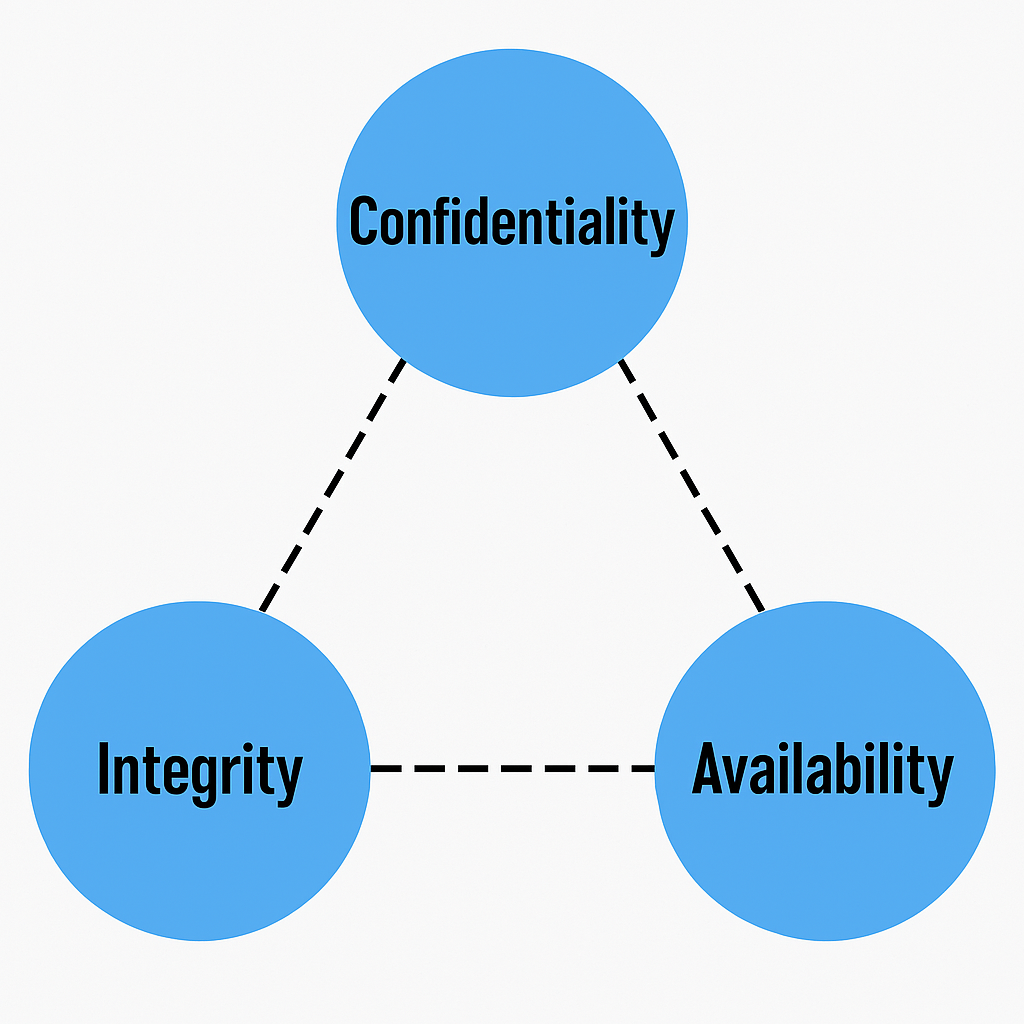
\includegraphics[width=0.5\linewidth]{figures/Triada_Seguridad.png}
            \caption{Triada de la seguridad}
            \label{fig:Triada-Seguridad}
        \end{figure}

        El \textbf{criptoanálisis} es la ciencia  —y en ocasiones, el arte—, de descifrar criptosistemas sin conocer previamente la clave. El criptoanálisis es de vital importancia para los criptosistemas modernos, ya que sin el análisis constante por parte de expertos que intenten vulnerarlos, no sería posible determinar si dichos métodos son verdaderamente seguros \cite{paar_understanding_2010}.
            
        La \textbf{criptografía clásica} -también conocida como criptografía precuántica- se basa en algoritmos cuya seguridad radica en problemas matemáticos considerados intratables para los ordenadores convencionales. Estos algoritmos han resistido con éxito numerosos intentos de criptoanálisis a lo largo del tiempo. Entre los más representativos se encuentran:
            \begin{itemize}
                \item \textbf{RSA}, basado en la factorizacion de numeros enteros muy grandes.
                \item \textbf{Elliptic Curve Cryptography (ECC)}, que utiliza el logaritmo discreto en curvas elípticas.
            \end{itemize}
            
        La criptografía se divide, a su vez, en tres ramas principales: 
            \begin{itemize}
                \item Algoritmos simétricos, utilizan una misma clave para cifrar y descifrar la información. Fueron el enfoque predominante desde los orígenes de la criptografía. Entre ellos, destaca AES por su eficiencia y robustez.
                    
                \item Algoritmos asimétricos, introducidos en 1976 por \textbf{Whitfield Diffie}, \textbf{Martin Hellman} y \textbf{Ralph Merkle}, emplean un par de claves: una pública (que se puede compartir) y una privada (que debe mantenerse secreta). Ejemplos clave son RSA y ECC.
                
                \item Protocolos criptográficos, combinan estos algoritmos para lograr funciones como el intercambio seguro de claves, la autenticación o la firma digital, siendo componentes esenciales en aplicaciones como VPNs, correo cifrado o blockchain.
                
            \end{itemize}

            El cifrado simétrico habilita una comunicación segura sobre un canal de transmisión inseguro, asumiendo que la clave secreta se comparte sobre un canal seguro. 

            \begin{figure}[h]
                \centering
                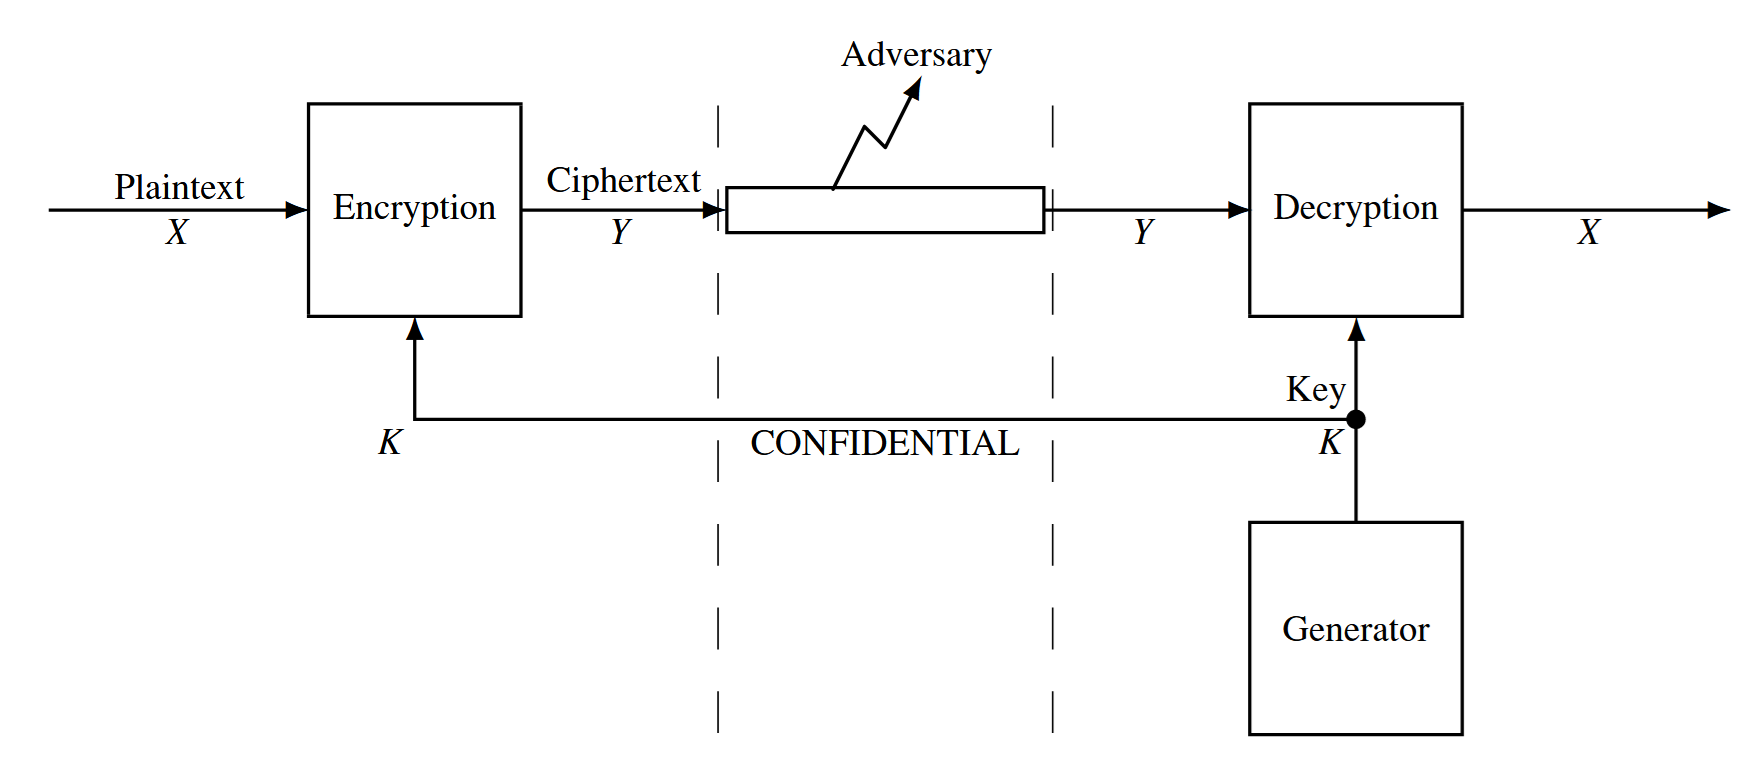
\includegraphics[width=1\linewidth]{figures/Simetric.png}
                \caption{Cifrado Simétrico}
                \label{fig:cifrado-Simétrico}
            \end{figure}

            En la Figura~\ref{fig:cifrado-Simétrico} se observa cómo la clave secreta se transmite del receptor al transmisor de una manera confidencial, mientras que el atacante intenta obtener la información cifrada. 

            El \textbf{estándar avanzado de cifrado (AES, por sus siglas en inglés)} es uno de los algoritmos de cifrado simétrico más utilizados en la actualidad. Se ha convertido en un componente esencial de numerosos sistemas y protocolos de seguridad ampliamente desplegados, tales como IPsec, TLS, SSH, y el cifrado de redes Wi-Fi mediante el estándar IEEE 802.11i. Hasta la fecha, no se ha descubierto ningún ataque criptográfico práctico más eficiente que la fuerza bruta, lo que lo convierte en una opción robusta y confiable para proteger información confidencial \cite{paar_understanding_2010}. AES soporta bloques de datos de 128 bits y admite claves de 128, 192 o 256 bits. Gracias a esta solidez, AES sigue siendo a día de hoy el estándar predominante para el cifrado simétrico en la mayoría de los sistemas modernos.

            Por otro lado, los cifrados asimétricos -también conocido como criptosistemas de clave publica- está definido por tres algoritmos, un generador de claves pseudoaleatorios, que produce un par de claves (publica $K_p$, y una privada $K_S$); un algoritmo de cifrado, que puede ser probabilístico y produce un cifrado $Y$ a partir del mensaje $X$ y la clave publica; y un algoritmo de descifrado, que es determinista y recupera el mensaje original $X$ a partir del cifrado $Y$ y la clave secreta.

            \begin{figure}[h]
                \centering
                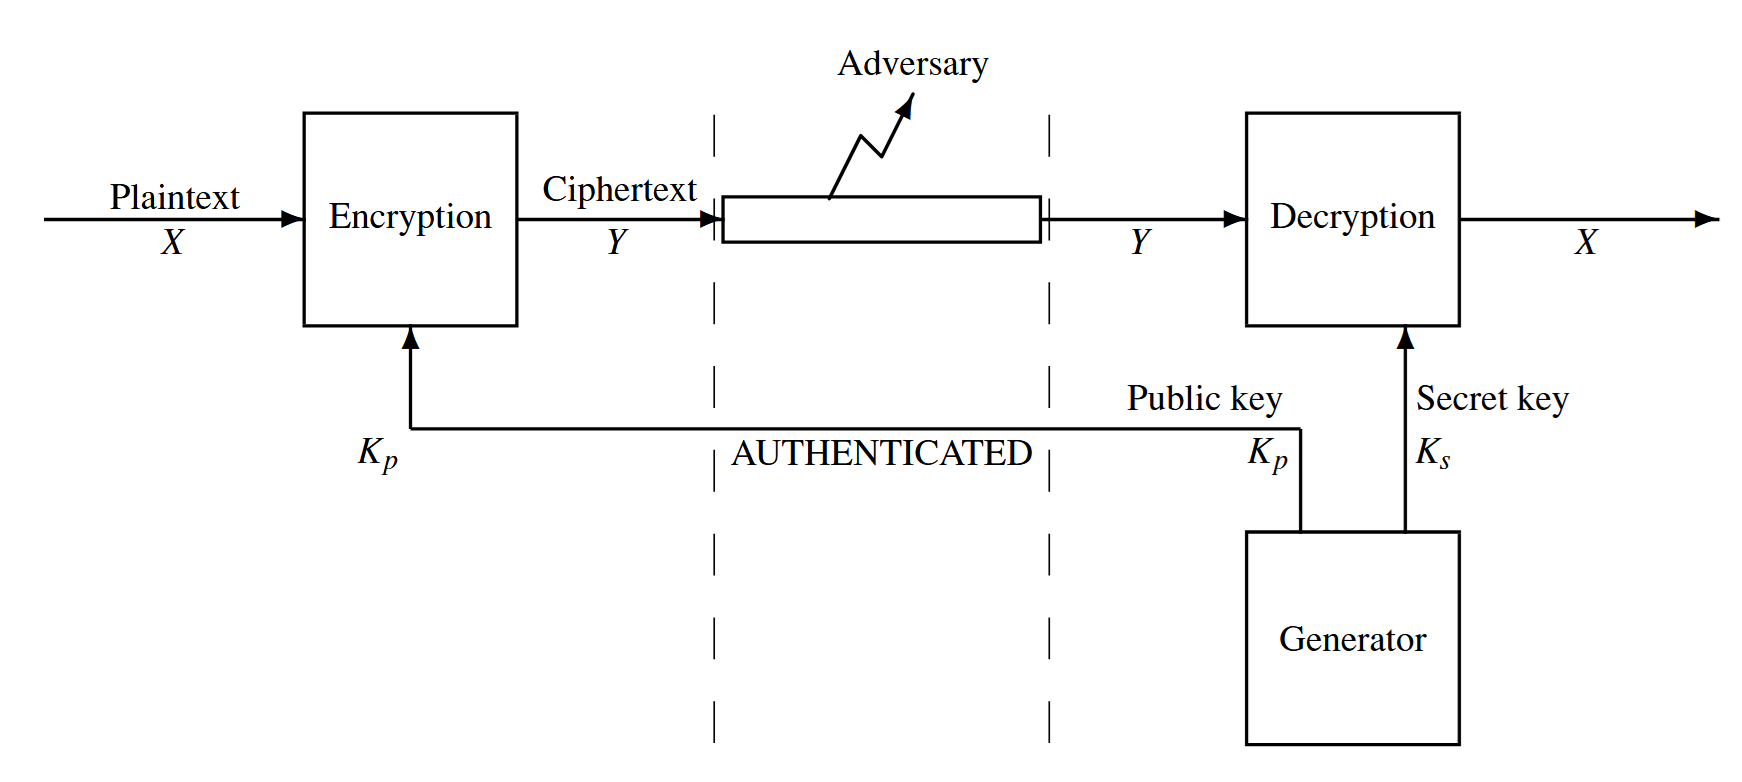
\includegraphics[width=1\linewidth]{figures/Asimetric.png}
                \caption{Cifrado Asimétrico}
                \label{fig:Cifrado-Asimetrico}
            \end{figure}

            Figura~\ref{fig:Cifrado-Asimetrico} se muestra un modelo de sistema asimétrico en el que el texto plano se encripta con una 
            clave publica y descifrada con la llave secreta. Es importante destacar, que aun con el acceso a la clave publica, 
            debe ser computacionalmente intratable recuperar el mensaje sin consultar la llave privada. 

            Aunque los algoritmos clásicos, han demostrado ser eficientes durante décadas, el desarrollo de la computación 
            cuántica plantea nuevas amenazas que comprometen su seguridad. Lo que ha impulsado las investigaciones en nuevos 
            esquemas resistentes a ataques cuánticos.  

            Para entender como la computación cuántica puede romper los esquemas criptográficos clásicos, debemos entender sus dos principales algoritmos: \textbf{Shor} y \textbf{Grover}. 
            El algoritmo de Shor, desarrollado por Peter Shor en 1994 \cite{SHOR}, demuestra que los ordenadores cuánticos pueden resolver dos problemas matemáticos de especial complejidad,
            que los ordenadores clásicos no pueden resolver en un tiempo razonable: la factirización de números enteros y el calculo de logaritmos discretos. 
            Ambos problemas constituyen la base de la seguridad de sistemas criptográficos de clave pública. Shor muestra que se pueden resolver mediante algoritmos cuánticos cuyo
            tiempo de ejecución crece de manera polinómica con el tamaño de entrada.

            Este resultado es relevante para RSA. La seguridad de RSA depende de la dificultad de obtener los facotres primos de un número entero grande. El algoritmo de Shor
            transforma el problema de factorización en otro problema, denominado \textit{Busqueda del orden}. Para un entero $x$ coprimo con $N$, se busca el menor entero positivo
            $r$ que satisface:

            \begin{equation}
                x^r \equiv 1 \mod N
            \end{equation}

            Una vez que se encuentra el periodo $r$, es posible calcular factores de $N$ utilizando algoritmos clásicos como el maximo común divisor (\textbf{MCD}). 

            La ventaja cuántica de Shor se encuentra en un registro que puede representar una \textit{superposición de muchos valores simultáneamente}. Shor utiliza
            esta propiedad junto con operaciones de exponenciación modular y la \textit{Transformada Cuántica de Fourier (\textbf{QFT})}. La QFT permite extraer
            información sobre el periodo existente en los estados cuánticos, que constituye el núcleo del algoritmo. 

            Además, Shor desarrolla el algoritmo para resolver el problema del logaritmo discreto. Dado un generador $g$ y un valor $x$, se busca el entero $r$ que satisface:
            
            \begin{equation}
                g^r \equiv x \mod p
            \end{equation}

            El algoritmo muestra también que se puede resolver mediante la exponenciación modular y la QFT, obteniendo un algoritmo eficiente en un ordenador cuántico. Esta segunda
            aportación es tan relevante como la primera: implica que los sistemas cuya seguridad depende del logaritmo discreto, como el Diffie-Hellman y, por extensión, los sistemas
            basados en curvas elípticas, también son vulnerables. 

            Shor no demuestra que un ordenador cuántico es "más rapido". Demuestra que ciertos problemas matemáticos, en los que se basan los sistemas criptográficos de clave pública
            clásica cambian de complejidad cuando se dispone de un ordenador cuántico. 

            Por otro lado, Lov K. Grover, en 1996 \cite{grover}, desarrolló un algoritmo que permite buscar un elemento en una lista desordenada de $N$ elementos. Si no existe ninguna estructura
            que permita saber dónde se encuentra el elemento buscado, un algoritmo clásico debe revisar cada elemento de la lista. Lo que en promedio requiere:

            \begin{equation}
                \frac{N}{2} \text{ iteraciones}
            \end{equation}

            En términos de complejidad, el problema requiere:

            \begin{equation}
                O(N) \text{ iteraciones}
            \end{equation}

            Por lo tanto, el algoritmo proporciona una \textit{aceleración cuadrática} respecto a los algoritmos clásicos. Grover señala que existe un límite inferior
            de $\Omega(\sqrt{N})$ para este tipo de búsquedas cuánticas, por lo que el algorimo de Grover es los más eficiente posible.

            La idea fundamental del algoritmo de Grover es representar simultáneamente mendiante superposición cuántica todos los posibles estados del espacio de búsqueda. 
            Inicialmente, los $N$ posibles elementos reciben la misma amplitud:

            \begin{equation}
                \frac{1}{\sqrt{N}}
            \end{equation}

            De esta manera, ningún elemento tiene inicialmente una probabilidad mayor que los demás de ser observados. 

            Existe una operación que permite identificar el estado correspondiente a la solución sin medir directamente el sistema. Esta función, se suele describir como \textit{Oráculo},
            modifica la fase del estado que cumple la condición de búsqueda:

            \begin{equation}
                |x\rangle \rightarrow -|x\rangle
            \end{equation}

            cuando $x$ es la solución, mientras que los demás estados permanecen sin modificar. Después se aplica la \textit{transformación de difusión}, conocida como \textit{Grover diffusion operator},
            que modifica las amplitudes de los estados de manera que la amplitud asociada a la solución aumenta, mientras disminuyen las amplitudes
            de los demás estados. 

            El proceso tiene una complejidad de:

            \begin{equation}
                O(\sqrt{N}) \text{ iteraciones}
            \end{equation}

            Después de las iteraciones, la probabilidad de medir el estado buscado es suficientemente alta como para recuperar la solución. 

            Supongamos una clave simétrica de $n$ bits. Existen:

            \begin{equation}
                N = 2^n \text{ posibles claves}
            \end{equation}

            Por fuerza bruta, a un atacante le tomaria $2^{n}$ intentos encontrar la clave correcta. Sin embargo, al aplicar Grover:

            \begin{equation}
                O(\sqrt{2^n}) = O(2^{\frac{n}{2}}) \text{ iteraciones}
            \end{equation}

            Es decir, de manera idealizada, la seguridad efectiva frente a búsqueda exhaustiva se reduce aproximadamente a la mitad en términos de bits. 
            
            Como se mencioná en \cite{european_union_agency_for_cybersecurity_post-quantum_2021}, la computación cuántica es una inovación disruptiva extremadamente poderosa, 
            que tiene el potencial de romper los esquemas criptográficos de clave publica ampliamente utilizados, como se demostró anteriormente. Mientras que no sabemos cuando 
            los ordenadores cuánticos estarán disponibles, los investigadores y autoridades institucionales están trabajando en soluciones. Como resultado, \textbf{NIST}, aun esta en proceso de estandarización de algoritmos criptográficos resistentes a ataques cuánticos.

            Debemos hacer la distinción entre criptografía post-cuántica (\textbf{PQC}) y criptografía cuántica. PQC se basa en diseñar soluciones criptográficas que se pueden usa en los
            ordenadores no cuánticos, que creemos que pueden resistir criptoanalisis tanto cuanticos como convencionales. Por otro lado, la criptografía cuántica se basa en soluciones
            criptográficas que toman ventaja de las propiedades de la física cuántica para proporcionar ciertos servicios de seguridad, como la distribución de claves cuánticas (\textbf{QKD}).
            
            En el trabajo de Schöffel et al \cite{schoffel_code-based_2022} se define la criptografía basada en códigos (\textit{code-based cryptography}) como una familia de criptografía post-cuántica
            cuya seguridad se apoya en la dificultad de resolver detrerminados problemas asociados a los códigos correctores de errores. Estos códigos se utilizan originalmente para detectar y corregir 
            errores durante la transmisión de información, pero tambien pueden emplearse para construir sistemas criptográficos cuando el proceso de decodificación resulta computacionalmente difícil 
            para un atacante. 

            En términos generales, estos esquemas introducen de forma controlada errores en la información codificada. El receptor legítimo dispone de la estructura necesaria para corregirlos, 
            mientras que un atacante debe enfrentrarse a un problema de decodificación mucho más complejo. Sin embargo, las implementaciones basadas en códigos suelen presentar una mayor complejidad
            computacional y mayores requsitos de memoria. 

            Dentro de esta familia se encuentra \textbf{HQC}, que combina un código decodificable con un código aleatorio de estructura doblemente circulante. Esto permite reducir el tamaño 
            de las claves respecto a otros esquemas basados en códigos. 


    \subsection{HQC}
    
    HQC (\textit{Hamming Quasi-Cyclic}) es un mecanismo de encapsulación de claves post-cuántico basado en códigos. Su objetivo no es cifrar directamente todos los datos de una aplicación, sino 
    permitir que dos participantes establezcan de forma segura un secreto compartido, que después es capaz de emplearse con criptografía simétrica como AES. La especificación distingue entre \textbf{HQC-PKE}, el esquema
    de cifrado de clave pública subyacente, y \textbf{HQC-KEM}, que construye sobre el mecanismo de encapsulación. Según \cite{noauthor_hamming_nodate}.

    La seguridad de HQC se basa en el \textbf{Quasi-Cyclic Syndrome Decoding Problem} (\textbf{QCSD}), un problema de la teoría de códigos. Conceptualmente, el atacante conoce cierta información 
    sobre un código y debe recuperar un vector de errores de pequeño peso de Hamming. Para ciertos parámetros, encontrar ese vector es computacionalmente complicado. La especificación usa variantes 
    más concretas de este problema, como \textbf{2-DQCSD-P} y \textbf{3-DQCSD-PT}. La estructura \textit{Quasi-Cyclic} permite representar matrices mediante vectores y rotaciones circulantes, reduciendo así
    el espacio necesario para almacenar claves frente a una representación aleatoria. HQC trabaja fundamentalmente sobre vectores binarios que pueden interpretarse como polinomios en el anillo:
    
    \begin{equation}
        R = \frac{\mathbb{F}_2[X]}{(X^n - 1)}
    \end{equation}
    
    Es por ello, que muchas de las operaciones de HQC terminan siendo sumas, multiplicaciones y rotaciones sobre grandes vectores binarios. 

    El peso de Hamming indica cuántas posiciones de un vector binario son distintos de cero. HQC genera diferentes vectores secretos y de error con pesos de Hamming controlados. 
    Estos errores son los que introducen la dificultad criptogáfica, se deben escoger de tal manera que el receptor legítimo siga siendo capaz de corregirlos. HQC incorpora un código auxiliar basado en \textbf{Reed-Muller} y \textbf{Reed-Solomon}. Su función es permitir recuperar el mensaje a pesar del ruido introducido durante el cifrado. 

    HQC se entiende mediante tres operaciones:

    \begin{itemize}
        \item KeyGem
        \item Encaps
        \item Decaps
    \end{itemize}

    Para comenzar el proceso de establecer un sistema seguro, uno de los participantes debe generar una clave pública y privada segura, esto se le conoce como \textbf{KeyGen},
    para generar estas claves se usan vectores aleatorios de peso reducido y estructura cuasi-cíclica de HQC.

    Una vez que la clave pública se hace llegar al segundo participantge, este genera un valor aleatorio, construyendo lo que se conoce como \textbf{Ciphertext} empleando la clave pública e introduce los vectores
    de error adicionales, este proceso se conoce como \textbf{Encaps}. En este proceso se obtiene también el \textit{secreto compartido}.

    Finalmente, al hacerle llegar el \textit{Ciphertext} al primer paticipante, comienza un proceso de decodificación (\textbf{Decaps}) del esquema en el que se emplea la clave privada para recuperar la información necesaria y reconstruir exactamente
    el mismo secreto compartido.

    El resultado de este proceso resulta en que ambos extremos terminan obteniendo:

    \begin{equation}
        K_A = K_B
    \end{equation}

    Después de obtener el secreto, puede utilizarse para derivar claves simétricas. 

    Actualmente, HQC proporciona tres conjuntos de seguridad:

    \begin{itemize}
        \item HQC-1,
        \item HQC-3,
        \item HQC-5
    \end{itemize}

    correspondientes respectivamente a los niveles de seguridad NIST 1, 3 y 5. Estos conjuntos controlan aspectos como $n$, $n_1$, $n_2$, $k$, $\omega$, 
    $\omega_r$, $\omega_e$.

    De manera simplificada:

    \begin{itemize}
        \item $n$ determina el tamaño principal de los vectores utilizados.
        \item $n_1$ y $n_2$ están relacionados con el código concatenado de corrección de errores.
        \item $k$ determina el tamaño de la información codificada.
        \item $\omega$, $\omega_r$ y $\omega_e$ determinan los pesos de Hamming de distintos vectores secretos o de error.
    \end{itemize}

    A medida que aumenta el nivel de seguridad, estos valores aumentan, por lo que aumenta también el tamaño de \textit{las claves}, \textit{el ciphertext} y \textit{el coste computacional.}

    Por lo que hemos visto, HQC presenta un coste computacional significativo, la implementación en C de referencia necesita, para \textbf{HQC-1}, aproximadamente:
    $4.577$ x $10^6$ ciclos para KeyGen, $9.116$ x $10^6$ ciclos para Encaps, y $13.918$ x $10^6$ ciclos para Decaps. Sin embargo, los benchmarks se realizan sobre un 
    \textbf{Intel Core i7-11850H}, por lo que no llegan a representar el comportamiento en microcontroladores. 

    En arquitecturas ARM Cortex-M4, el coste de HQC está condicionado por las operaciones de multiplicación de polinomios binarios.
    Por ello, la optimización de estas operaciones permite reducir significativamente el número de ciclos necesarios para
    KeyGen, Encaps y Decaps, como se menciona en \textit{Optimized implementation of HQC on Cortex-M4} %\cite{Optimized implementation of HQC on Cortex-M4}.

    \subsection{Sistemas embebidos e IoT}
    



    \subsection{Criptografía post-cuántica en sistemas embebidos e IoT}
    
\section{Trabajos Relacionados}
    \subsection{Code-based Cryptography in IoT: A HW/SW Co-Design of HQC}
    \subsection{pqm4: Testing and Benchmarking NIST PQC on ARM Cortex-M4}
    \subsection{Optimized Implementation of HQC on Cortex-M4}
    \subsection{Post-Quantum Cryptography for Internet of Things: A Survey on Performance and Optimization}
    \subsection{A Comparative Study of Post-Quantum Cryptosystems for Internet-of-Things Applications}


\section{Objetivos}

El presente trabajo estudia la implementación de esquemas de seguridad post-cuánticos en sistemas embebidos para IoT, 
con el fin de evaluar su rendimiento en esta clase de entornos. Es por ello que se plantean una serie de objetivos 
que permiten estructurar el desarrollo de este proyecto. 

\begin{enumerate}
    \item Analizar el funcionamiento interno del esquema \textbf{HQC}
    \item Implementar el esquema \textbf{HQC} en un entorno IoT
    \item Evaluar el rendimiento del esquema HQC en terminos de ejecucion, consumo de memoria, y tamaño de clave/cifrado en el sistema elegido.
    \item Identificar posibles limitaciones y oportunidades de mejora para aplicaciones reales en dispositivos de bajo consumo
    \item Evaluar la sobrecarga que introduce el uso del esquema HQC en las comunicaciones, en comparación con un sistema sin cifrado post-cuántico.
\end{enumerate}
